\documentclass{beamer}
\usetheme{Boadilla}
\setbeamertemplate{navigation symbols}{}
%\usepackage[utf8x]{inputenc}
\usepackage[light]{antpolt}
\usepackage{hyperref}
\usepackage{tikz}
\DeclareMathOperator{\M}{\mathcal M}
\DeclareMathOperator{\N}{\mathcal N}
\DeclareMathOperator{\G}{\mathcal G}
\newcommand{\eq}[1]{\begin{align*} #1 \end{align*}}
\newcommand{\game}[8]{\eq{\begin{array}{ccccccccc} \text{I} & #1 && #3 && #5 && #7\\ \text{II} && #2 && #4 && #6 && #8 \end{array}}}
\newcommand{\reveal}[3][10]{\only<#3-#1>{\alert<#3>{\makebox[0pt][l]{$#2$}}}\phantom{#2}}
\newcommand{\dotss}{\makebox[0pt][l]{\dots}\phantom{\dots}}

\title[Games and Ramsey-like cardinals]{Games and Ramsey-like cardinals\\ {\small\textsc{Set Theory Today conference, Vienna}}}
\author[Dan Saattrup Nielsen]{Dan Saattrup Nielsen\\ University of Bristol}
\date{September 14, 2018}

\begin{document}

\begin{frame}
	\titlepage
\end{frame}

\begin{frame}{Let's play a game $\G_\alpha^\theta(\kappa)$}
  \game{\onslide<2->{\alert<2>{\M_0}}}{\onslide<3->{\alert<3>{\mu_0}}}{\onslide<4->{\M_1}}{\onslide<5->{\mu_1}}{\onslide<6->{\alert<6>{\cdots}}}{\onslide<6->{\alert<6>{\cdots}}}{\onslide<7->{\M_\alpha}}{\onslide<8->{\mu_\alpha}}
  
  \begin{enumerate}
    \item \onslide<2->{$\alert<2>{\M_\eta}\prec H_\theta$ is a $\kappa$-sized model of $\textsf{ZFC}^-$ containing $\kappa{+}1$}
    \item \onslide<3->{$\alert<3>{\mu_\eta}$ is an $\M_\eta$-normal $\M_\eta$-measure on $\kappa$ such that $\text{Ult}(\M_\eta,\mu_\eta)$ is wellfounded}
    \item \onslide<4->{The $\M_\eta$'s and $\mu_\eta$'s are \alert<4>{$\subseteq$-increasing}}
    \item \onslide<5->{We take \alert<5>{unions} at limit rounds}
    \item \onslide<7->{The game lasts for \alert<7>{$\alpha{+}1$ rounds}}
    \item \onslide<8->{\alert<8>{Player II wins} iff they can continue playing all rounds}
    \item \onslide<9->{\alert{\textsc{Important remark:}} The $\mathcal M_\eta$'s are \textbf{not} necessarily transitive!}
  \end{enumerate}
\end{frame}

\begin{frame}{Yet another large cardinal notion?!}
  \begin{block}{Definition\only<1-2>{ (Holy-Schlicht '18)}}\pause
    For $\alpha\leq\kappa$, a cardinal $\kappa$ is\textbf{\only<3>{\alert<3>{ weakly}} \alert<2>{strategic $\alpha$-Ramsey}} if,\\ for all regular $\theta>\kappa$, player II has a strategy in $\G_\alpha^\theta(\kappa)$ which is always winning\only<3>{\alert<3>{ the first $\alpha$ rounds}}.
  \end{block}
\end{frame}

\begin{frame}{What are the \alert<1>{finite versions} good for?}
  \begin{block}{Definition}
    Let $\kappa$ be a cardinal. Then
      \begin{itemize}
        \pause\item $\kappa$ is \textbf{weakly compact} if \only<7->{$\kappa\to(\alert<7>{[\kappa]^\kappa})^2$}\only<2-6>{$\alert<4>{\kappa}\to(\alert<5>{\kappa})^{\alert<6>{2}}$}\only<3-7>{, i.e. that for every colouring $c:[\alert<4>{\kappa}]^{\alert<6>{2}}\to\{0,1\}$ of \alert<6>{2}-element subsets of $\alert<4>{\kappa}$ into two colours there's a \textbf{homogeneous} }\only<7>{$X\in\alert<7>{[\kappa]^\kappa}$}\only<3-6>{$X\subseteq\kappa$ of size $\alert<5>{\kappa}$}\only<3-7>{; that is, all pairs of $X$ have the same\\ colour: $|c``[X]^2|=1$.}
        \onslide<9->\item $\kappa$ is \textbf{ineffable} if $\kappa\to(\{\text{stationary subsets of $\kappa$}\})^2$
        \onslide<10->\item $\kappa$ is \textbf{completely ineffable} if there's a non-empty upwards-closed set $R\subseteq\mathcal P(\kappa)$ consisting of stationary subsets of $\kappa$, such that $A\to(R)^2$ for every $A\in R$
      \end{itemize}
  \end{block}

  \only<11-13>{\begin{block}{Theorem (Abramson-Harrington-Kleinberg-Zwicker '77)}
    Let $\kappa=\kappa^{<\kappa}$ be a cardinal. Then
      \begin{itemize}
        \onslide<12-13>\item $\kappa$ is strategic $0$-Ramsey $\Leftrightarrow$ $\kappa$ is weakly compact
        \onslide<13>\item $\kappa$ is strategic $1$-Ramsey $\Rightarrow$ $\kappa$ is ineffable ($\Rightarrow$ $\kappa$ is strategic $0$-Ramsey)
      \end{itemize}
  \end{block}}

  \only<14->{\begin{block}{Theorem (N.)}
    A cardinal $\kappa$ is weakly strategic $\omega$-Ramsey iff $\kappa$ is completely ineffable.
  \end{block}}

  \only<15->{The proof uses the previous theorem as the base case. In the ``$\Leftarrow$'' direction, care must be taken at successor stages to ensure that the measures cohere.}
\end{frame}

\begin{frame}{What are the \alert<1>{countable versions} good for?}
  \begin{block}{Definition (Gitman-Schindler '16; original definition from Schindler '00)}
    A cardinal $\kappa$ is \textbf{remarkable} if \pause to every regular $\lambda>\kappa$ there is a regular $\nu>\lambda$ and a transitive $M$ closed under $\lambda$-sequences such that, in a generic extension, there's an elementary embedding $\pi:H_\nu^V\to M$ with $\text{crit }\pi=\kappa$ and $\pi(\kappa)>\lambda$.
  \end{block}
  
  \only<3>{
  \vspace{0.5cm}
  \begin{center}
    \begin{tikzpicture}

      % Labels 
      \node at (0,-0.5) {$H_\nu^V$};
      \node at (6.4,-0.5) {$M\supseteq {^\lambda}M\cap V$};
      \node at (2.9,-0.8) {$\pi$};
      \node at (-0.3,2.5) {$\nu$};
      \node at (-0.3,1.7) {$\lambda$};
      \node at (5.9,1.7) {$\lambda$};
      \node at (-0.3,0.9) {$\kappa$};
      \node at (6.1,2.9) {$\pi(\kappa)$};
       
      % Models
      \draw (0,0) -- (0,2.5);
      \draw (5.5,0) -- (5.5,3.5);
     
      % Ordinal markers
      \draw (-0.1,2.5) -- (0.1,2.5);
      \draw (-0.1,1.7) -- (0.1,1.7);
      \draw (-0.1,0.9) -- (0.1,0.9);
      \draw (5.4,2.9) -- (5.6,2.9);
      \draw (5.4,1.7) -- (5.6,1.7);

      \draw[dotted] (0,1.7) -- (5.5,1.7);
      
      % Embedding
      \draw[->] (0.5,-0.5) -- (5,-0.5);
      \draw[|->] (0.3,0.9) -- (5.2,2.9);

    \end{tikzpicture}
  \end{center}
  }

  \only<4>{
    \begin{block}{Proposition (Schindler '00)}
      Remarkable cardinals are downwards absolute to $L$.
    \end{block}
  }

  \only<5-8>{\begin{block}{Theorem(s)}
    The existence of a remarkable cardinal is equiconsistent with..
      \begin{enumerate}
        \onslide<6->\item (Schindler '00) proper forcing cannot change the theory of $L(\mathbb R)$
        \onslide<7->\item (Schindler '04) semi-proper forcing cannot change the theory of $L(\mathbb R)$
        \onslide<8->\item (Cheng-Schindler '15) $3^{rd}$ order number theory + Harrington's Principle (``there is a real $x$ such that every $x$-admissible ordinal is an $L$-cardinal")
      \end{enumerate}
  \end{block}}
  
  \only<9->{\begin{block}{Theorem (Schindler-N.)}
    Every remarkable cardinal is strategic $\omega$-Ramsey, and if $\kappa$ is strategic $\omega$-Ramsey then either $\kappa$ is remarkable in $L$ or
      $$ L_\kappa\models\text{There is a proper class of strategic $\omega$-Ramseys}. $$
  \end{block}}

  \only<10>{Consequently, strategic $\omega$-Ramseys are equiconsistent with remarkables.}

  \only<11>{The proof goes via the notion of a so-called \textit{virtually measurable cardinal}.}
\end{frame}

\begin{frame}{What are the \alert<1>{uncountable versions} good for?}
  \pause\begin{block}{Proposition}
    Every measurable cardinal $\kappa$ is strategic $\kappa$-Ramsey.
  \end{block}

  \only<3>{
    \alert{Proof}: In $\G_\kappa^\theta(\kappa)$ simply play the measure on $\kappa$.\qed
  }

  \only<5-11>{
    \begin{block}{Theorem (Welch '18)}
      Every strategic $\omega_1$-Ramsey cardinal $\kappa$ is measurable in the core model $K$ below the sharp of a strong cardinal, $0^\P$.
    \end{block}
  }
  \only<6-10>{
    \alert<6->{Proof sketch.} \onslide<7-> Jump to $V^{\text{Col}(\omega_1,\kappa^{+K})}$, let $\eta_\alpha\to\kappa^{+K}$ and let player I in $\mathcal G_{\omega_1}^\theta(\kappa)^V$ play models 
$$\mathcal M_\alpha:=\onslide<8->{\text{Hull}^{H_\theta^V}(}K|\eta_\alpha\onslide<8->{).}$$
Player II follows their winning strategy.

\onslide<9-> \qquad The final measure $\mu_{\omega_1}$ is then a $K$-measure and we can wlog assume that $\mu_{\omega_1}$ is countably complete and weakly amenable.

\onslide<10-> \qquad Then, since we're below $0^\P$, inner model theory magic (``the beaver argument'') implies that $\mu_{\omega_1}\in K$ and we're done.\qed
  }

  \only<12->{
    \begin{block}{Theorem (\alert{Schindler} '18)}
      Every strategic $\omega_1$-Ramsey cardinal $\kappa$ is measurable in the core model $K$ below \alert{a Woodin cardinal}.
    \end{block}
  }

    \only<11-12>{Strategic $\omega_1$-Ramseys are therefore equiconsistent with measurables.}
    \only<13>{The proof is similar, but different inner model theory magic is used.}
\end{frame}

\begin{frame}{So what happens between $\omega$ and $\omega_1$?}
  \begin{block}{Definition}
    A cardinal $\kappa$ is \textbf{Ramsey} if $\kappa\to(\kappa)^{<\omega}$.
  \end{block}
 
  \pause\begin{block}{Facts}
    \begin{enumerate}
      \item If there exists a Ramsey cardinal then $V\neq L$.
      \pause\item Measurable cardinals are Ramsey limits of Ramsey cardinals.
    \end{enumerate}
  \end{block}

  \pause\begin{block}{Theorem (Mitchell '79, Dodd '82)}
    A cardinal $\kappa$ is Ramsey iff every $A\subseteq\kappa$ can be put into a $\kappa$-sized model $M\models\textsf{ZFC}^-$ containing $\kappa{+}1$ such that there exists a weakly amenable countably complete $M$-measure on $\kappa$.
  \end{block}

\pause\begin{block}{Proposition (N.)}
    Strategic $(\omega{+}1)$-Ramsey cardinals are Ramsey limits of Ramsey cardinals.
  \end{block}
\end{frame}

\begin{frame}{So what happens between $\omega$ and $\omega_1$?}
  \only<1-4>{\begin{block}{Theorem (Mitchell '79, Dodd '82)}
    A cardinal $\kappa$ is Ramsey iff every $A\subseteq\kappa$ can be put into a $\kappa$-sized model $M\models\textsf{ZFC}^-$ containing $\kappa{+}1$ such that there exists a weakly amenable countably complete $M$-measure on $\kappa$.
  \end{block}}

\begin{block}{Proposition (N.)}
    Strategic $(\omega{+}1)$-Ramsey cardinals are Ramsey limits of Ramsey cardinals.
  \end{block}

  \pause\alert{Proof sketch.} Whenever $\vec{\mathcal M_\alpha}*\vec{\mu_\alpha}$ is a play of $\mathcal G_{\omega+1}^\theta(\kappa)$ then
$$ (\mathcal M_{\omega+1},\in,\mu_{\omega+1})\models\text{$\mu_{\omega+1}$ is countably complete}.$$

\pause Then $\mu_\omega\subseteq\mu_{\omega+1}$ implies that, wlog,
$$ \mathcal M_{\omega+1}\models\text{$\mu_\omega$ is countably complete and weakly amenable},$$

making $\mu_\omega$ countably complete and weakly amenable by elementarity.

\pause\qquad So $\kappa$ is Ramsey. \pause\pause But then $\mathcal M_\omega\models\text{$\kappa$ is Ramsey}$ and so $\text{Ult}(\mathcal M_\omega,\mu_\omega)\models\text{$\kappa$ is Ramsey}$, since $\mathcal M_\omega$ has the same subsets as the ultrapower by weak amenability of $\mu_\omega$.

\pause\qquad \L o\' s and elementarity then makes $\kappa$ a limit of Ramseys.\qed

\end{frame}


\begin{frame}{Alright then. What about when we exceed $\omega_1$?}
  \begin{block}{Proposition (N.)}
    Let $\lambda$ be uncountable regular. Then $\kappa$ is strategic $\lambda$-Ramsey iff \pause there's a ${<}\lambda$-closed forcing $\mathbb P$ such that, in $V^{\mathbb P}$, there's a transitive $N$ with $\mathcal P(\kappa)^V=\mathcal P(\kappa)^N$ and an elementary embedding $j:V\to N$ with $\text{crit}(j)=\kappa$.
  \end{block}

  \only<3>{\vspace{0.5cm}\begin{center}
    \begin{tikzpicture}

      % Labels 
      \node at (-0.7,-0.5) {${^{<\lambda}}V\subseteq V$};
      \node at (5.5,-0.5) {$N$};
      \node at (2.9,-0.8) {$j$};
      \node at (6.1,2.5) {$j(\kappa)$};
			\node at (6.2,1.5) {$\kappa^{+N}$};
      \node at (-0.3,0.9) {$\kappa$};
			\node at (-0.7,1.5) {$\kappa^{+V}$};
       
      % Models
      \draw (0,0) -- (0,3);
      \draw (5.5,0) -- (5.5,3);
      
      \draw[dotted] (0,1.5) -- (5.5,1.5);
     
      % Ordinal markers
      \draw (-0.1,0.9) -- (0.1,0.9);
      \draw (-0.1,1.5) -- (0.1,1.5);
      \draw (5.4,1.5) -- (5.6,1.5);
      \draw (5.4,2.5) -- (5.6,2.5);
      
      % Embedding
      \draw[->] (0.5,-0.5) -- (5,-0.5);
      \draw[|->] (0.3,0.9) -- (5.2,2.5);

    \end{tikzpicture}
  \end{center}}

  \onslide<5->{\begin{block}{Theorem (Schindler-N.)}
    The ``$\Rightarrow$'' direction in the $\lambda=\omega$ case above.
  \end{block}}

  \onslide<6>The ``$\Leftarrow$'' direction is open --- getting wellfoundedness of $\text{Ult}(\mathcal M_\omega,\mu_\omega)$ seems hard. We've shown it in the case where $N\subseteq V$.
\end{frame}

\begin{frame}{What's not known?}
  \begin{block}{Question 1}
    Are the strategic $\alpha$-Ramseys equivalent to some kind of ``generic embedding property" when $\alpha$ is countably infinite, as in the uncountable regular case?
  \end{block}
  
  \pause\begin{block}{Question 2}
    Do the strategic $\alpha$-Ramseys form a strict hierarchy for $\alpha$ countably infinite? More specifically, does
$$\textsf{ZFC}+\exists\text{strategic $(\alpha{+}1)$-Ramsey}\vdash\text{Con}(\exists\text{strategic $\alpha$-Ramsey})?$$
  \end{block}
  
\end{frame}

\begin{frame}{An overview}
  \begin{center}
    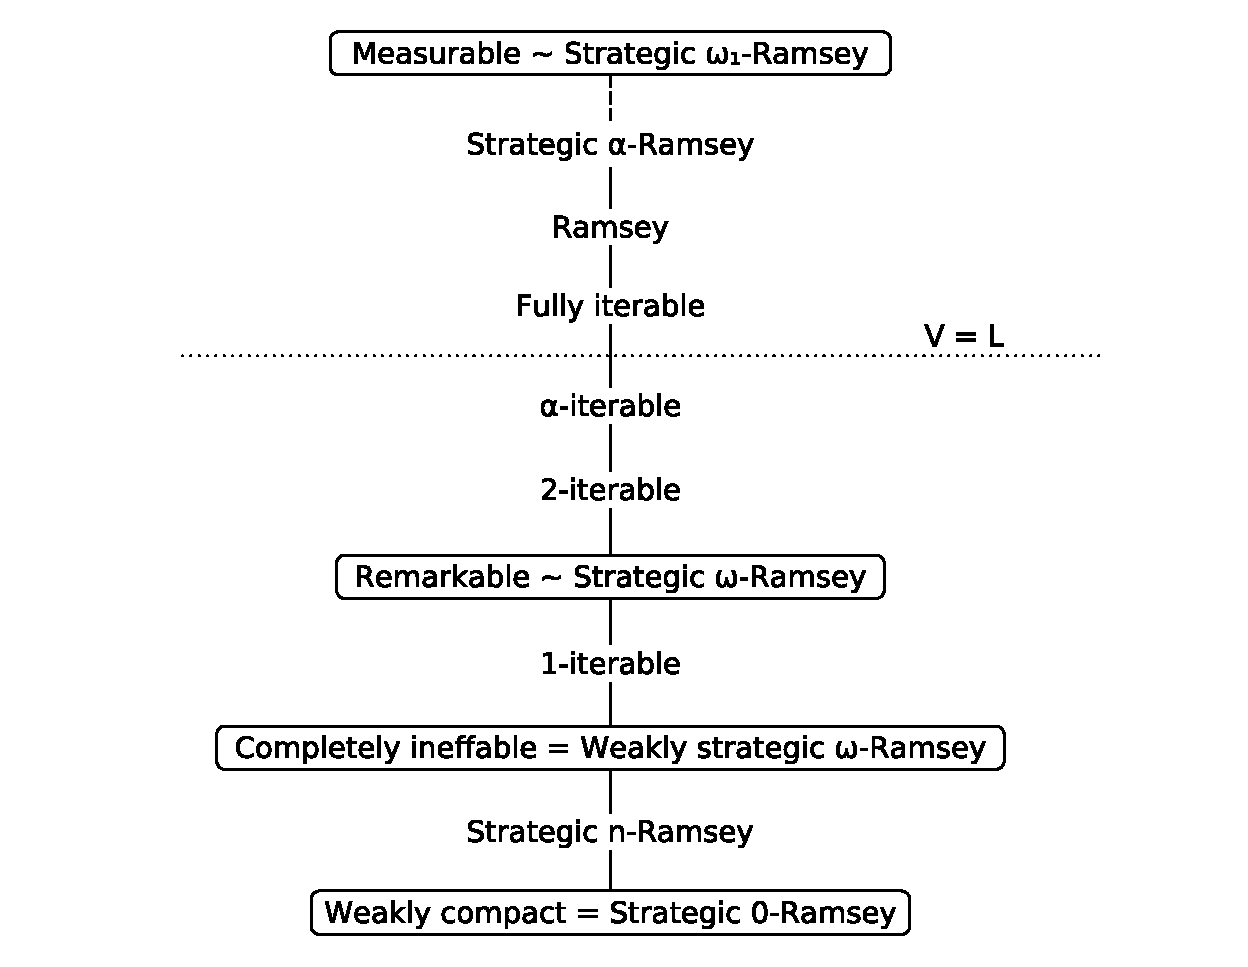
\includegraphics[scale=0.48]{gfx/diagram.pdf}
  \end{center}
\end{frame}

\begin{frame}{}
  \begin{center}
    {\Large Thank you for your attention}\\\vspace{1.5cm}
    Slides and preprint available at\\
    \url{https://dsnielsen.com}
  \end{center}
\end{frame}

\end{document}
